% \lstset{style=mystyle}
\section{Register File}
The Register File serves as a source for operands and a destination for storing results during arithmetic or logical operations. In instruction execution, the processor reads operands from the register file, performs operations, and writes results back to it.\newline
\subsection{Overview and Code implementation}
 We see that the Register File has as an input a clock signal, 3 addresses, InDataA, UpdateFlags and InNewFlags. For outputs we have We have OutDataB and C, OutFlags, and we also added a DebugData wire that we used to test our module and show the content of the registers. We have declared 3 Addresses for our input because our simplified RISC-V processor has 3 formats for instruction where RI type calls only one register, RRI type calls 2 registers and RRR types calls 3.\newline
\begin{figure}[H]
                \centering
                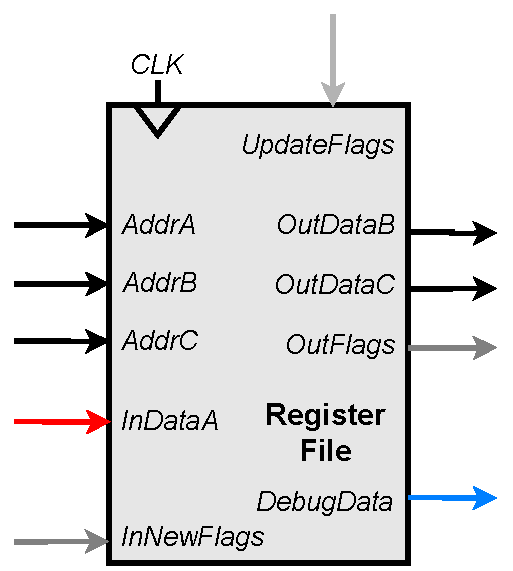
\includegraphics[width=.2\textwidth]{pics/diagrams/riscv/modules/register_file}
                \caption{Register file diagram}\
\end{figure}
After the input and output declaration, we specified that $R_7$ -- flags register using the following parameter:
\begin{code}[20]{Flags Register address}
	parameter FlagsAddress = 7;
\end{code}

Then we declared an array of registers named Data. This array consists of eight 16-bit registers which will be initialized to zero. \newline

This part is concerned with the read functionality of the Register File where we assign the data stored at the address specified by AddrB to OutDataB and we do the same for AddrC and OutDataC. We also assign the data stored in FlagsAddress to OutFlags. This allows us to read the content of the registers.\newline
\begin{code}[32]{Read functionality}
    assign OutDataB = Data[AddrB];
	assign OutDataC = Data[AddrC];
	assign OutFlags = Data[FlagsAddress[2:0]];
\end{code}
On the other hand, this section is responsible for the write functionality where on the positive edge of the clock signal, the block triggers and writes the input data InDataA into the register specified by AddrA. Also, if UpdateFlags is asserted, it updates the flags data stored at the address specified by FlagsAddress with the new flags data InNewFlags.\newline

\begin{code}[37]{Write functionality}
    always @ (posedge Clk) begin
		Data[AddrA] = InDataA;

		if (UpdateFlags)
		Data[FlagsAddress[2:0]] = InNewFlags;
	end
\end{code}
This final part has been added mainly for debugging and testing our Register File.\newline

Overall, our module implements a simplified register file with read and write functionality, flags update capability, and debug output for monitoring register content while operating synchronously with the clock signal.\newline